\part{Cours Magistral 1 -- Les intégrales multiples}
\section*{Introduction}
\emph{Livre de référence : Calculus Adams}
Les théorèmes ne sont pas démontrés par manque de temps mais ils sont tout de même intéressants.
\section{Intégrales multiples}

Cette section se réfère au chapitre 14 du livre de référence.
\subsection{Introduction}
\[\int_{a}^{b} {f(x) dx}\]


\begin{enumerate}

\item Partition P du domaine $D=[a,b]$
$$ P = \{x_0,x_1,\dots,x_n\}$$
$$a=x_0<x_1<\dots<x_n=b$$
\item On définit la norme de P
$$||P|| = \underset{1\le i \le n}{\max} \overbrace{(x_i-x_{i-1})}^{\Delta x_i}=1$$

\item Dans chaque $[{x_{i-1},x_i}]$ : on choisit un point $c_i$ avec $c=(c_1,c_2,\dots,c_n)$

\item  Somme de Riemann : $$R(f,P,c)=\sum_{i=1}^{n} \overbrace{f(c_i)\dot \Delta  x_i}^{\textbf{aire du rectangle i}} $$

\item Passage à la limite $$\lim\limits_{\substack{||P|| \to 0 \\ n \to \infty}} R(f,P,c) =\int_{a}^{b} {f(x) \dif x}$$

\end{enumerate}
Si cette limite existe, quels que soient les points $c_i$, alors on dira que cette fonction est intégrable.
\begin{myrem}
$$\int_{a}^{b} {f(x) \dif x} = \int_{a}^{b} {f(t) \dif t} = \int_{a}^{b} {f(\alpha) \dif \alpha}$$ où $f(x)$ représente l'intégrand et $\dif x$ représente la variable d'intégration \textit{\og dummy variable \fg{}}.
\end{myrem}

\begin{myrem}

Les courbes sous l'axe sont négatives et au-dessus sont positives. On additionne le tout. On peut donc avoir une somme d'aire négative.

$$\int_{a}^{b} {f(x) \dif x} \quad D=[a,b] \subset \mathbb{R}^1$$
$$\int_D f(x_1,x_2,\dots,x_n) \dif x_1 \dots \dif x_n \quad D \in \mathbb{R}^n$$
La généralisation de $n=1$ à $n=2$ n'est pas évidente, mais la généralisation de $n=2$ à $n=\infty$ est plus simple, étrangement.
\end{myrem}

\subsection{Intégrale Double}
\includegraphics[scale=1]{image3.png}

Région solide $ S \subset \mathbb{R}^3$
\[I=\int \limits_{D} f = \iint_D f (x,y) \dif A\]
$\dif A$ est un élément d'aire infinitésimale. L'écriture avec une seule intégrale et uniquement l'intégrant est la notation \og matheuse\fg{}, l'écriture avec autant d'intégrales que de dimensions, et avec le $\dif A$, est la notation \og ingénieur\fg{}.

$(f \ge 0) \Rightarrow I = \text{Volume de S}$

Développons un peu\dots
\begin{enumerate}
\item

$$D= \text{``pavé'' dans }\mathbb{R}^2 = [a,b]\times[c,d]$$

Chaque rectangle est appelé $R_{ij}$, avec \(1 \le i \le m\) et \(1 \le j \le n\)

$$R_{ij}=[x_{i-1},x_i]\times[y_{j-1},y_j]$$
L'aire de $R_{ij}$ vaut donc
$$R_{ij}=[x_{i-1},x_i] \cdot [y_{j-1},y_j]= \Delta x_i \Delta y_j$$

\item{Norme de P}

diag = diamètre $R_{ij}= \sqrt{\Delta x_i^2+\Delta y_j^2}$


\item


\textit{Dans chaque $R_{ij}$, on choisit un point}
$$\{c_{ij}^* = (x_{ij}^*,y_{ij}^*)\} = C^*$$

\item
$$R(f, P,c^*)=\sum_{i=1}^{m} \sum_{j=1}^{n} f(x_{ij}^*,y_{ij}^*)\Delta A_{ij}$$
Avec $\Delta A_{ij}$ qui vaut $\Delta x_i \Delta y_j$

\item

$$\lim\limits_{\substack{\norm{P} \to 0 \\ n \to \infty\\ m \to \infty}} R(f,P,c^*)=\int_D f$$

\end{enumerate}

\begin{mytheo}

Si f est continue sur $D$, alors f est intégrable sur $D$. C'est vrai aussi pour toutes les dimensions ! C'est une condition suffisante (l'inverse n'est pas vrai).

C'est-à-dire une fonction non-continue peut être intégrable.

\end{mytheo}

\subsection{ Généralisation à $D$ borné }

\subsubsection{ Dans $ \mathbb{R}^2$ }

\includegraphics[scale=1]{image4.png}

Rectangle qui contient le domaine D et dont les côtés sont parallèles aux axes.
\[\hat{f} = \text{ extension f de D à } \mathbb{R^2}\]

\[
\hat{f}(x,y)
\begin{cases}
f(x, y) & \text{si } (x, y) \in D \\
0 & \text{sinon} \\
\end{cases}%\left\{
%\begin{array}{l r}
%f(x,y)\text{ si }(x,y)\in D\\
%0\text{ sinon}\\
%\end{array}
%\right.
\]

$f$ intégrable sur D $ \Longleftrightarrow \hat{f}$ intégrable sur $\mathbb{R^2}$ et alors
$\int_D f \eqdef \int_R \hat{f} $


On peut appliquer maintenant pour $n$ :
\\
$ D \subset \mathbb{R}^n$
$$\int_D f = \overbrace{\iint \dots}^\text{$n$-uple} \int_D f(x_1,x_2,\dots,x_n) \dif x_1 \dif x_2 \dots \dif x_n $$

Le produit des $\dif x_1 \dots \dif x_n $ qui sont des éléments infinitésimaux de volume

\subsubsection{Dans $\mathbb{R}^3$}

D = boite de $\mathbb{R}^3$ avec les faces parallèles aux plans de coordonnées\\

Il faut faire un découpage en sous-boîtes $ R_{ijk} $ de taille $\Delta x_i \Delta y_j \Delta z_k$

$\left\{
\begin{array}{l}
1 \le i \le m \\
1 \le j \le n \\
1 \le k \le l \\
\end{array}
\right. $

Il faut choisir \[C_{ijk}^* \in R_{ijk} ( x_{ijk}^*,y_{ijk}^*,z_{ijk}^*)\]

\[R(f,P,c^*)=\sum_{i=1}^m \sum_{j=1}^n\sum_{k=1}^l f (x_{ijk}^*,y_{ijk}^*,z_{ijk}^*) \Delta V_{ijk}\]

On aura donc que

$$\lim\limits_{\substack{l \to \infty \\ n \to \infty\\ m \to \infty}} R=\int_D f$$

Solide borné de $\mathbb{R}^3$
\[\hat{f}=
\begin{cases}
f & \text{si } (x, y, z) \in D \\
0 & \text{sinon} \\
\end{cases}
\]

\[\int_D f \eqdef \int_R \hat{f}\]
\emph{
Donc, lorsque le domaine de définition d'une intégrale est borné dans $\mathbb{R}^2$ ou $\mathbb{R}^3$, on peut étendre ce domaine à condition de poser que les points qui n'appartiennent pas à ce domaine valent $0$.}
\subsection{Propriétés}

\[\int_D f \text{ avec D borné sur } \mathbb{R}^n\]

\begin{myprop}
$f\equiv 1 $
\[\text{D borné de }\mathbb{R}^n\]
\[n=1 : D=[a,b] \int_a^b 1 = b-a = \text{Longueur de }D\]
\[n=2 : D=[a,b]\times[c,d] \int_a^b \int_c^d 1 = (b-a) \cdot (d-c)= \text{Aire de }D\]

\[n=3 : \int_D 1 = \text{Volume de }D\]

Et ainsi de suite. Il suffit d'intégrer la fonction $f(x) = 1$ pour connaître la longueur, la surface, le volume, etc. du domaine.
\end{myprop}


\begin{myprop}
$\forall L,M \in \mathbb{R} ,\forall f,g$ intégrable sur $D \subset \mathbb{R}^n$


\[\int_D(Lf+Mg)\overset{?}{=}L\int_D f + M \int_D g\]
On effectue un déplacement linéaire de l'intégrale. L'intégrale étant une fonction linéaire, cette égalité est justifiée !

\end{myprop}


\begin{myprop}
$$\text{Si } f \le  g  \text{ } \forall \text{ point de }D\subset \mathbb{R}^n \text{alors} \int_D f \le \int_D g $$
Cette propriété se vérifie très facilement de manière géométrique.
\end{myprop}

\begin{myprop}
$D= D_1 \cup D_2 \cup \cdots \cup D_k$ et $D_i \cup D_j = \varnothing$ et $i\neq j$ non-overlapping

On aura donc que l'intégrale sur $D_i$ de $f$ est
\[\int_D f=\sum_{j=1}^k \int_{D_j} f\]

On peut découper le domaine D en plusieurs sous-domaines distincts et calculer la somme des intégrales sur chacun des sous-domaines.
\end{myprop}

\begin{myprop}
\[\abs{\int_D f} \le \int_D\abs{f}\]

La valeur absolue de l'intégrale de f sera toujours plus petite que l'intégrale de la valeur absolue de f. Encore une fois, on voit cela très rapidement de manière géométrique. C'est une généralisation de l'inégalité triangulaire.
\end{myprop}

\begin{myprop}[Théorème de Fubini :]
\emph{Ce théorème ne se trouve pas dans le livre !}
Il permet de \strong{réduire} le calcul d'une intégrale $n$-uple à une \strong{succession} (dans l'ordre qui convient le mieux) de n intégrales \strong{unidimensionelles}.

\textit{\textbf{Enoncé}} \\Soit $f$ définie sur un pavé D de $\mathbb{R}^n$\\
$D=[a_1,b_1]\times[a_2,b_2]\times \cdots\ \times[a_n,b_n]$

\[f(x_1,x_2,\cdots,x_n) : D\to\mathbb{R}\]
Si $f$ est continue sur D, alors : $(\sigma(1),\sigma(2),...,\sigma(n)) $ = une permutation quelconque de (1,2,...,n)

$$
\int_D f= \int_{a_{\sigma(1)}}^{b{\sigma(1)}}
\left[
\int_{a_{\sigma(2)}}^{b{\sigma(2)}}
\left[ \cdots\ \left[
\int_{a_{\sigma(n)}}^{b{\sigma(n)}}
f(x_1,x_2,\cdots,x_n )\dif x_{\sigma(n)}
\right]\cdots\right]
\dif x_{\sigma(2)} \right] \dif x_{\sigma(1)}
$$

Si la fonction f est \textbf{continue}, on peut calculer les intégrales les unes après les autres dans l'ordre de notre choix en considérant les autres variables comme des constantes.
\end{myprop}




\subsubsection{Illustration du Théorème de Fubini pour $n=2$}




$ \left\{
\begin{array}{l}
D = [0,2]\times[1,3]\\
f = x^2+y
\end{array}
\right.
$

$
 \left\{
\begin{array}{l}
x_1=x\\
x_2=y
\end{array}
\right.
$
$(1,2)=(\sigma(1),\sigma(2))$

\[\int_D f = \int_0^2 \left[ \overbrace{\int_1^3 (x^2+y) \dif y}^{\text{Intégrale interne}}\right] \dif x\]

A l'intérieur, c'est ``\textit{y}'' qui est la variable d'intégration et ``\textit{x}'' est considéré comme constant.

\[=x^2\int_1^3 \dif y+\int _1^3 y \dif y = x^2 \cdot 2+\left.\frac{y^2}{2}\right]_1^3 = 2x^2+4\]

Au final, l'intégrale vaudra donc
\[  \int_0^2(2x^2+4)dx = 2\frac{x^3}{3}+4x \left]_{(2,0)} \right.= 40/3\]
On va maintenant vérifier si, en intégrant dans l'ordre inverse, on obtient le même résultat.
\[I = \int_1^3 \left[ \int_0^2 (x^2+y)\dif x \right] \dif y\]

A l'intérieur, on a \[\frac{x^3}{3}+2y = 8/3 + 2y\]

Au final, on aura donc \[I = \int_1^3(\frac{8}{3}+2y)\dif y = 40/3\]

Le théorème de Fubini fonctionne !

\begin{myrem}
Notation des physiciens\\
Exemple :
$$\left\{
\begin{array}{l}
\int_0^2\dif x\int_1^3\dif y (x^2+y)\\
\int_1^3\dif y\int_0^2 \dif x ( x^2+y)
\end{array}
\right.
$$
On lit à l'envers, c'est-à-dire de droite à gauche.
\[\int_D f = \int_{a_{\sigma(1)}}^{b{\sigma(1)}} \dif x_{\sigma_1} \cdots \int_{a_{\sigma(n)}}^{b{\sigma(n)}} \dif x_{\sigma_n} f(x_1 \cdots x_n)\]

\end{myrem}

\subsection{Méthodes de calcul de l'intégrale double}
\subsubsection{Par inspection : $(D,f)$}
Exemple 1 :

\[I=\int_D 3 \text{ sur le domaine }D=[a,b]\times[c,d]\]
\[I=3\int_D 1 = 3 \cdot \text{Surface de }D = 3\overbrace{(d-c)(b-a)}^{\text{Surface de }D} \]

Autre exemple :
\[I = \int_D ( \sin(x) +y^3 + 4 )\text{ sur le domaine } D=x^2+y^2\le 1\]
\[I = \iint_D(\sin(x)+y^3+4)\dif x\dif y = \int_D \sin(x) + \int_D y^3 + \int_D 4 = I_1 + I_2 + I_3\]
\begin{itemize}

\item \textbf{$I_1$}




\[\sin(-x) = -\sin(x) \]
C'est une fonction impaire !
Donc on aura \emph{$I_1=0$}
Mais attention, le domaine doit être symetrique par rapport à l'axe y.
\item \textbf{$I_2$}
Pour la même raison, nous avons $I_2=0$ parce que $(-y^3) = -(y^3)$

\item \textbf{$I_3$}

L'intégrale devient donc
\[\int_D 4 = 4(\pi r^2) = 4\pi \]

\end{itemize}
\subsubsection{Utiliser/généraliser le théorème de Fubini}

Le domaine D est ``$y$-simple'' ou alors ``$x$-simple''\\
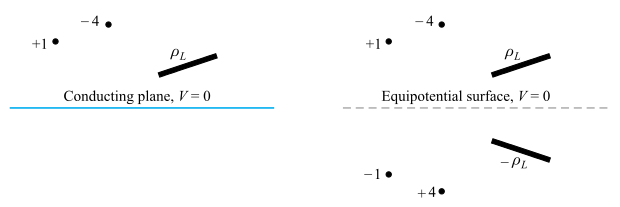
\includegraphics[scale=0.7]{image2.png}
\\
Les bords de la fonction pour y-simple sont $y=c(x)$ et $y=d(x)$.

Pour $x$-simple, c'est la même chose mais dans l'autre sens. Les bornes sont donc $x=a(y)$ et $x=b(y)$.
\begin{myrem}
$D$ peut être à la fois $x-$ et $y$-simple.
\end{myrem}
\begin{myrem}
Contre-exemple : Lorsqu'une des deux bornes n'est pas une fonction $y=d(x)$ ou $y=c(x)$, le domaine n'est pas y-simple. C'est la même chose pour x-simple.

\end{myrem}

\begin{myrem}
$D$ est ``régulier'' lorsqu'on peut trouver une union finie de domaines simples.


Par exemple, dans ce cas-ci, chacun des 4 sous-domaines est un domaine simple.\\
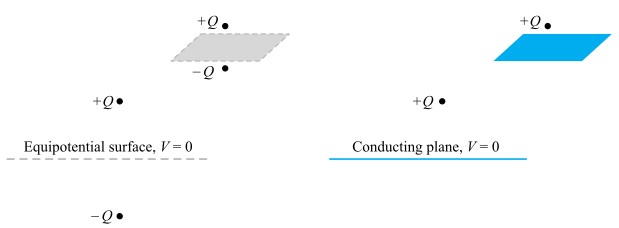
\includegraphics[scale=1]{image1.png}

\end{myrem}
